%%%%%%%%%%%%%%%%%%%%%%%%%%%%%%%%%%%%%%%%%%%%%%%%%%%%%%%%%%%%%%%%%%%%%%%%%%%%%%%%
% This chapter describes the text processing steps
%%%%%%%%%%%%%%%%%%%%%%%%%%%%%%%%%%%%%%%%%%%%%%%%%%%%%%%%%%%%%%%%%%%%%%%%%%%%%%%%
\chapter{Data Processing}
Data is received in a textual list of records consisting of meta data and the
text description of the complaint. We apply several processing steps to each
document to first extract the physical entity keywords, and then to calculate
the semantic scores. For this dataset, we have chosen the semantics of
occurrence relations and co-occurrence relations. Finally we segment \threed
models to match our keyword ontology. Each of the steps are explained in greater
detail below.


\section{Entity Vocabulary}
The first issue was to devise a method for extracting physical entities; a
document can contain multiple entities, but not all of which are related to the 
subject matter. On top of that, many entities can have implicit hierarchical 
relations, such as relation between component and its subcomponents. This 
relation is important because it enables logical groupings which are useful for
high level overviews.

Before any semantic processing can take place, we spent some time doing
preliminary analysis, looking at the data text, their format and how they have
evolved over the life span of the data repository. We performed several
normalization tasks: One, we used regular expressions to convert the text from
all capital cases to normal case format. Second, we remove suffix characters that
appear at the end of the text paragraph, that, as far as we know contributes
nothing to the incident context. Although we changed the underlying text, the
normalization process improves readability, and enables us to receive more
meaningful outputs from natural language parsers.

\subsection{Keyword Hierarchy}
Our entity extraction process leverages the WordNet database, a lexical English
database that stores nouns, verbs, adjectives and their relations among each
other \cite{WORDNET}. In order to get a comprehensive list of physical entities, we use the meronym 
relation in WordNet. A meronym describes a ``part-of'' relationship between two 
nouns, for example, a brake is a part of a wheel, and a wheel is a part of the 
automotive vehicle. All together, the meroynomy relationship forms a hierarchical 
structure where the most general part forms the root node, while the most specific 
parts form the leaf nodes. We use two common words pertaining to the subject
matter of our dataset to bootstrap the creation of the hierarchy hierarchy:
``car'' and ``vehicle''. From this, we recursively extracted children entities
using the meronomy relationship until we have two tree structures, which we then
merged together.

While this process extracts a fair amount of physical entities, an analysis of
sample dataset showed that it is not a representative of the entities mentioned
in the documents. The primary reason for this is due to the use of synonyms
in the document text. To alleviate this situation, we additionally extract
the synset relations from WordNet for each keyword. A synset is a set
relationship that describes words that are semantically equivalent of one
another, for example ``limo'' and ``limousine'' are different words, but both
describe the same type of object and thus belongs to the same semantic group.
For each word in our current vocabulary, we replace it with the its synset.


    % ===== Figure =====
	\begin{figure}
	   \centering  
	   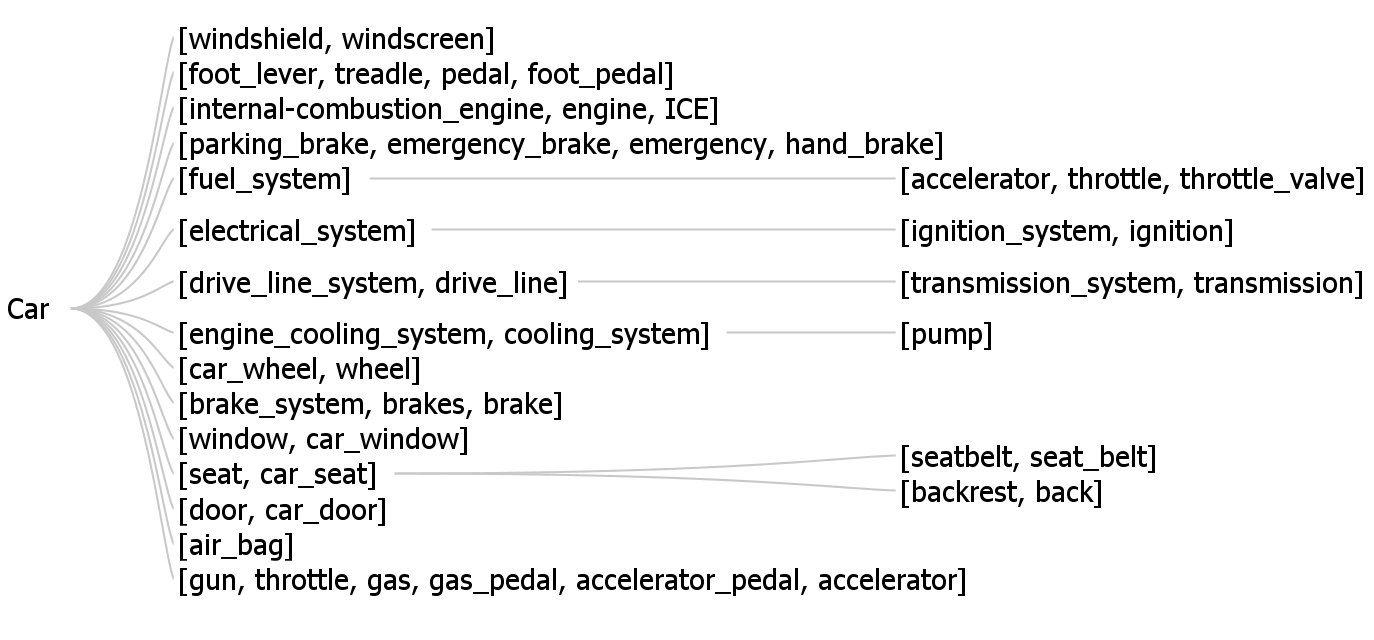
\includegraphics[width=\columnwidth]{meronomy.png}
	   \caption{An example of the meronomy plus synset structure}
	   \label{figure:meronomy}
	\end{figure}
	% ==================


\subsection{Refinement}
The addition of synsets into the vocabulary gave us a comprehensive number of
keywords, however it also created undesirable noises. Manual examination of data
sample reveals that there are still disconnects between the dictionary
vocabulary and real world vocabulary. As an additional step to augment our
keyword vocabulary, we perform two manual steps:

\begin{itemize} [noitemsep]
  \item Removal of nouns that are too generic from the vocabulary.
  \item Preprocess the documents and mine for any missing nouns.
\end{itemize}
The first step deals with the removal of keywords that are not considered to be
physical objects under typical usage, for example WordNet hierarchy of a
vehicle contains ``first'', ``second'', ``third'' and ``fourth'', which
describes the first, second, third and fourth gears respectively. Including
these words will likely result in over-counting the number of occurrences of
gears because they are used in every day speech, but not typically with respect
to car gears. We also removed several acronyms that will likely cause
ambiguities, for example ``ICE'', which is short for internal-combustion-engine,
will cause issues if the document is about ice, the solid state of water. They
are therefore removed from the keyword vocabulary.

The second step deals with any possible missing keywords that are not in WordNet
meronym synsets. We attempted to detect these semi-automatically with natural
language processing techniques. We first perform part-of-speech (POS) tagging on our document 
corpus. POS taggers look at the grammatical structures of text and break down 
sentences into lexical categories such as nouns, verbs and adjectives. We use the 
POS output and tie them back to the original text, extracting the nouns and 
compound-nouns. We perform this step for all the documents in the corpus and 
count the number of occurrences for the nouns and compound-nouns. We then manually 
exam the top occurring nouns and add them into the hierarchy where we believe 
would be appropriate.

\subsection{Limitations}
While we believe this extract process is a plausible method for building the
vocabulary, we acknowledge that WordNet is not the definitive authority for our 
problem domain, nor would it be for any specific domain. The automatic
extraction can be used as a starting point. The keywords vocabulary should be
extended and further refined by consulting experts that works in the problem field. 



\section{Semantic Relations}
We chose to look at two semantic relations in our dataset: occurrence and
co-occurrence relations. The occurrence relation is a measure of how frequently
a particular entity was mentioned throughout the corpus, and is an
indication how important the entity is overall. The co-occurrence relation is
also a frequency measure, it measures how frequently an entity is mentioned along
with other entities in the same document, indicating possible causal relations.
For example: ``Engine failed because radiator overheated'' has a co-occurrence
relation between engine and radiator.

Semantic relations are defined as document-entity pairs, that is to say, there
is a one-to-many relation between a document and our keyword ontology. Detection of
keywords in document is done through a tagging process. In the sections below we
describe this process in detail, as well as formalizing the semantic scoring
function.
 

\subsection{Tagging}
%We use straight forward string matching to tag each document. 
Straight forward string matching is used for tagging of each document
First, document text is segmented into word tokens, then for each token we
search for a string match against the entity keywords. When a match is found, we
store a triple that describes the document identifier, the keyword and the
indexed position of the word in the document. In the aforementioned example
above, we would store
\emph{(Doc0, engine, 0)} for the engine entity, and \emph{(Doc0, radiator, 3)}
for the radiator entity.

In the actual string matching, we use an open source, off the shelf snowball
stemmer\footnote{http://snowball.tartarus.org/} to normalize each word token. 
Stemming is a process of reducing the words to their root forms. Finding the
root is important because it unifies the singular and plural forms, as well, it
converges various forms without the need to add additional vocabulary to our
keywords. We performed stemming on both the word tokens as well as our keyword
vocabulary.

For the document text, stemming is performed on all string tokens and not
limited to nouns. This has both positive and negative effects. In our data, 
there are many word tokens with both noun and verb forms, for example ``braking
malfunction'' can be correctly associated with the keyword ``brake'' with
stemming. On the other hand this also introduced false positives, the word
``lock'', which refers to the component, is falsely picked up when the text describe components
``locking up''.

In addition, we have also looked at tagging explicit casual relations. Using the
dependency parser extension, the output is a tree-like structure that can be used to infer
word dependencies. In practice this did not work very well; informal languages,
spelling mistakes and grammatical errors result in incorrect dependency parse
trees. We ultimately opted to go for a more general approach, where we tag each
physical entities as well as co-occurring entities within the same document.


\subsection{Scoring}
Once all documents are tagged, the occurrence and co-occurrence scores can be
computed. 

% Once we have identified the entities in each document, we can compute each
% entity�s importance score. We denote the importance score of a physical entity 
% as the number of times it is mentioned within the document corpus. We have two 
% variations of importance score: occurrence  and co-occurrence. Within our
% problem context, the occurrence scores denotes the components that are most prone to failure, while 
% the co-occurrence suggest causal relationships among the objects.

Let G be a (possibly empty) set of objects that are in the keyword hierarchy and
c be a single object in the hierarchy. We define a scoring function S(c, G) to be 
the total number of documents that have at least a single mention of c and G. Thus 
when G is the empty set the score is the occurrence score (every document 
contains an empty set). When G is non-empty the score reflects the co-occurrence 
strength among a set of components. For clarity we illustrate this with a few examples:
\begin{itemize} [noitemsep]
  \item $S(engine, \{\})$: The number of documents that mentions the entity
  engine.
  
  \item $S(engine, \{engine\}$): The number of documents that mentions the
  entity engine and engine, thus this is the same as above. 
  
  \item $S(engine, \{brake\})$: The number documents that mention both
  ``engine'' and ``brakes''. 
\end{itemize}

Each document is only counted once per physical entity, this was done to
discourage biases coming from longer documents where the entities are
repetitively mentioned.

Unlike the tagging process, scores are not stored, but rather
evaluated on a need basis. The numerous combinations that make up the set G
along makes it impractical to persist the scores in any manner, as the number of
possibilities is a permutation of all available entities.
 
Upon retrieving the entity scores during runtime, each score is normalized
to show relative strength with respect to each other. First, the system finds
the highest score within a subset of the data being visualized, then it uses the
score as a divisor so the scores are normalized to a range between 0 and 1.

  
\subsection{Limitations} 
For this prototype, we gave the same score weighting to each objects. This is a 
subjective measure because not all parts are created equal. For example: if window 
is mentioned 10 times and the engine mentioned a single time, does that mean we 
should pay more attention to the window component? A simple extension to this
work would be to devise an appropriate weighting scheme by consulting the domain
experts. 

Another limitation is the vocabulary set itself, while we are only storing nouns 
as keywords, it would be interesting to look at verbs as well. For example, 
``stalled'', ``stalling'' are typically associated with engine object. Adding
verbs into our dictionary would give more flexibility and accurate results.


\section{Model Segmentation}
We use geometric models that compose of triangular mesh groups, where each mesh 
group can be uniquely identified and semantically mapped to our keyword ontology. 
The segmentation is done manually, with consultation of car schematics when it 
was not clear where the parts located. Where the model is missing parts, 
we add placeholder geometries.

We have chosen to use a sedan model as the starting point of our visualization. 
This was chosen based on the fact that sedans are the most common class of 
vehicles and best represent our data. We acknowledge that different types of 
vehicles may have different spatial arrangement of their components, we hope to 
remedy this as more vehicle models are processed.

